\begin{pastexam}[label={px:df3-106-ds-01}]{地方三等資訊處理 106 年 第一題}
（申論；30 分）

給定一個以一維陣列 A[i]所表示的二元樹（binary tree）如下：（每小題 5 分，共 30 分）
\begin{center}
\begin{tabular}{|c|*{15}{c|}}
\hline
i & 1 & 2 & 3 & 4 & 5 & 6 & 7 & 8 & 9 & 10 & 11 & 12 & 13 & 14 & 15 \\
\hline
A[i] & T & S & U & B & O & G & & & & & P & X & & & \\
\hline
\end{tabular}
\end{center}
\begin{enumerate}[leftmargin=2.2em]
\item[㈠] 請問該樹樹高為何？
\item[㈡] 請列舉該樹所有葉節點（leaf node）。
\item[㈢] A[i]所代表的節點之左子節點（left-child node）應在陣列 A[.]的那一個位置？請寫出公式。
\item[㈣] 請寫出該樹之後序遍歷（Postorder Traversal）結果。
\item[㈤] 請寫出該樹之前序遍歷（Preorder Traversal）結果。
\item[㈥] 請寫出該樹之中序遍歷（Inorder Traversal）結果。
\end{enumerate}
\end{pastexam}

\begin{pastsoln}
\textbf{還原樹。} 陣列從 1 開始存，A[$i$] 的左子在 A[$2i$]、右子在 A[$2i+1$]，父節點在
A[$\lfloor i/2 \rfloor$]（資結書第~7.2.1~節）。 有值的位置是 1--6、11、12：
\begin{itemize}
\item A[1]$=$T 是根，左子 A[2]$=$S、右子 A[3]$=$U。
\item S（2）：左子 A[4]$=$B、右子 A[5]$=$O。 U（3）：左子 A[6]$=$G，右子 A[7] 空。
\item B（4）：A[8]、A[9] 都空，是葉節點。 O（5）：A[10] 空，右子 A[11]$=$P。 G（6）：左子 A[12]$=$X，
A[13] 空。
\item P（11）、X（12）的子節點在 22--25，超出陣列，都是葉節點。
\end{itemize}
\begin{center}
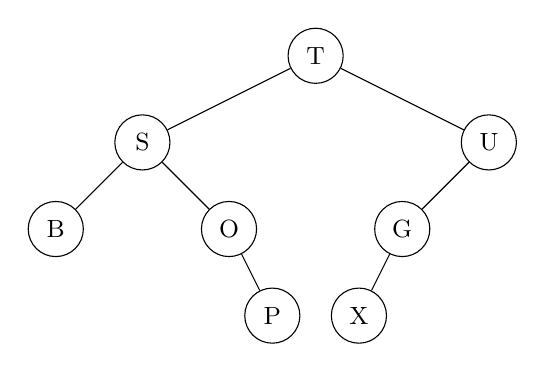
\begin{tikzpicture}[
    every node/.style={circle, draw, minimum size=7mm, inner sep=0pt, font=\small},
    level distance=11mm,
    level 1/.style={sibling distance=44mm},
    level 2/.style={sibling distance=22mm},
    level 3/.style={sibling distance=11mm}]
\node {T}
  child {node {S}
    child {node {B}}
    child {node {O}
      child[missing]
      child {node {P}}}}
  child {node {U}
    child {node {G}
      child {node {X}}
      child[missing]}
    child[missing]};
\end{tikzpicture}
\end{center}

\textbf{㈠ 樹高 4。} 最深的節點是 P（T--S--O--P）和 X（T--U--G--X），從根到它們共 4 個節點，所以有
4 層。 資結書第~7.1~節的樹高數的是層數（節點數）；若樹高定義成根到最深葉節點的\textbf{邊數}，答案是 3。
作答時寫明採用的定義。 也可以從陣列看：最大的編號 12 在第 $\lfloor \lg 12 \rfloor + 1 = 4$ 層。

\textbf{㈡ 葉節點：B、P、X。} 沒有任何子節點的節點。 O 只有右子 P、G 只有左子 X、U 只有左子 G，
都不是葉節點。

\textbf{㈢ 左子在 A[$2i$]。} 陣列從 1 開始時，第 $d$ 層的節點編號是 $2^{d-1}$ 到 $2^d - 1$，編號
$i$ 的節點前面同一層有 $i - 2^{d-1}$ 個節點，它們在下一層占了 $2(i - 2^{d-1})$ 個位置，所以 $i$ 的
左子編號是 $2^d + 2(i - 2^{d-1}) = 2i$，右子是 $2i + 1$。 （若陣列從 0 開始，左子是 $2i + 1$。）
本題例如 A[5]$=$O 的左子應在 A[10]（空的），A[6]$=$G 的左子在 A[12]$=$X。

\textbf{㈣ 後序（左、右、根）：B, P, O, S, X, G, U, T。}
左子樹 S：後序是 B, (O 的子樹：P, O), S，得 B, P, O, S；右子樹 U：(G 的子樹：X, G), U，得 X, G, U；
最後是根 T。

\textbf{㈤ 前序（根、左、右）：T, S, B, O, P, U, G, X。}

\textbf{㈥ 中序（左、根、右）：B, S, O, P, T, X, G, U。}
S 的子樹：B, S, 然後 O 的子樹（O 沒有左子）O, P；接著根 T；U 的子樹：G 的子樹 X, G，再 U（U 沒有右子）。
\end{pastsoln}
